\chapter{Células madre, regeneración y envejecimiento}\label{ch:b3:stem-cells}

Córtese la pata a un ajolote y en dos meses habrá crecido una nueva,
con hueso, músculo, nervio y piel en los lugares correctos, y volverá a
hacerlo tantas veces como se le corte. Córtese una planaria en veinte
trozos y cada uno se volverá un gusano entero en quince días, y el
trozo que era cola regenerará una cabeza con ojos y un encéfalo.
Córtese un dedo humano por encima de la última articulación y cicatriza
como una cicatriz. Y sin embargo el cuerpo humano no carece de
renovación: cada segundo fabrica dos millones de glóbulos rojos, el
revestimiento del intestino se sustituye cada cinco días y la piel cada
mes, y todo ello desciende de poblaciones pequeñas de células que se
dividen durante toda la vida sin agotarse. Este capítulo trata de esas
células ---qué hace a una \omterm{def:b3:stem-cells:stem}{célula madre}, cómo la conserva su \omterm{def:b3:stem-cells:stem}{nicho}, cómo
se construye a partir de ella toda la jerarquía de la sangre o del
intestino---, de los animales que pueden regenerar lo que nosotros no y
de por qué, del descubrimiento de que cualquier célula puede
devolverse al estado embrionario con cuatro genes, y de lo que la
aritmética de la división celular tiene que decir sobre por qué
envejecemos.

\section{Qué es una célula madre}

\begin{definition}[Las células madre y su jerarquía]\label{def:b3:stem-cells:stem}
\index{célula madre}\index{autorrenovación}\index{división asimétrica}\index{progenitor}\index{célula amplificadora de tránsito}\index{nicho}
Una \emph{célula madre} tiene dos propiedades que la definen: puede
\emph{autorrenovarse}, produciendo hijas que son células madre, y puede
producir hijas que se diferencian. Puede hacer ambas cosas a la vez,
por \emph{división asimétrica}, una hija de cada clase, con el destino
decidido por una herencia desigual de determinantes o por cuál de las
hijas sigue en contacto con el \emph{nicho} ---el microambiente de
células vecinas, matriz y señales que mantiene madre a una célula---; o
puede dividirse de forma simétrica, con unas divisiones que dan dos
células madre y otras que dan dos células que se diferencian, y la
población mantenida constante en promedio. Las hijas que se diferencian
suelen pasar por etapas de \emph{progenitor} o de \emph{amplificación
de tránsito}, en las que se dividen varias veces más con una potencia
cada vez más estrecha antes de madurar: la jerarquía amplifica unas
pocas divisiones lentas de célula madre hasta una producción grande, y
limita el número de divisiones que ha de hacer cada célula madre. Las
células madre adultas son raras y lentas ---una célula madre
hematopoyética se divide quizá una vez al año, y una célula madre
intestinal una vez al día--- y son \emph{multipotentes}, ceñidas a los
linajes de su tejido; las \omterm{def:b3:stem-cells:pluripotency}{células madre embrionarias}, de la masa
celular interna del blastocisto, son \emph{pluripotentes}, capaces de
hacer todos los tejidos del cuerpo pero no la placenta.
\end{definition}

\begin{omfigure}
\begin{tikzpicture}[every node/.style={font=\scriptsize}, >=stealth]
  \node[draw, very thick, rounded corners, fill=omDef!25, align=center] (hsc) at (0,3.6) {célula madre hematopoyética\\$\sim$\num{10000} en un ser humano; se divide $\sim$ una vez al año};
  \node[draw, thick, rounded corners, fill=omDef!12, align=center] (mpp) at (0,2.4) {progenitores multipotentes};
  \node[draw, thick, rounded corners, fill=omThm!15, align=center] (cmp) at (-3.2,1.2) {progenitor mieloide};
  \node[draw, thick, rounded corners, fill=omProp!20, align=center] (clp) at (3.2,1.2) {progenitor linfoide};
  \node[align=center, font=\tiny] (e) at (-5.4,-0.4) {eritrocitos\\$2\times 10^{11}$/día};
  \node[align=center, font=\tiny] (pl) at (-3.6,-0.4) {plaquetas\\(megacariocitos)};
  \node[align=center, font=\tiny] (g) at (-1.8,-0.4) {granulocitos\\$10^{11}$/día};
  \node[align=center, font=\tiny] (m) at (-0.2,-0.4) {monocitos,\\macrófagos};
  \node[align=center, font=\tiny] (b) at (1.8,-0.4) {linfocitos B};
  \node[align=center, font=\tiny] (t) at (3.4,-0.4) {linfocitos T};
  \node[align=center, font=\tiny] (nk) at (5.0,-0.4) {células NK};
  \draw[->, thick] (hsc) -- (mpp); \draw[->, thick] (mpp) -- (cmp); \draw[->, thick] (mpp) -- (clp);
  \foreach \x in {e,pl,g,m} { \draw[->, thick] (cmp) -- (\x); }
  \foreach \x in {b,t,nk} { \draw[->, thick] (clp) -- (\x); }
  \draw[->, thick, omDef!70!black] (hsc.west) .. controls (-3.0,4.4) and (-3.0,3.0) .. (hsc.south west) node[pos=0.5, left, font=\tiny, omDef!70!black, align=right] {autorrenovación};
  \node[right, align=left, font=\tiny] at (4.4,3.6) {cada piso se divide más a menudo\\y tiene una potencia más estrecha;\\$\sim 20$ divisiones de la célula madre\\al glóbulo rojo, de modo que una división\\de una célula madre rinde $\sim 10^{6}$ células};
\end{tikzpicture}

{\small La jerarquía hematopoyética. Unos pocos miles de \omterm{def:b3:stem-cells:stem}{células madre}
lentas de la médula alimentan \omterm{def:b3:stem-cells:stem}{progenitores} que se dividen deprisa y se
comprometen progresivamente, de modo que una producción de un billón de
células al día no cuesta a las \omterm{def:b3:stem-cells:stem}{células madre} casi nada.}
\end{omfigure}

\begin{proof}[Evidencia]
Till y McCulloch (1961) inyectaron células de médula en ratones
irradiados a dosis letal y contaron los nódulos que aparecían en el
bazo diez días después: cada uno era una colonia de células sanguíneas
de varios linajes, su número proporcional a las células inyectadas, y
marcar los cromosomas de las células donantes mostró que cada colonia
era un clon ---una sola célula había hecho glóbulos rojos, granulocitos
y plaquetas, y algunas colonias contenían células capaces de sembrar
colonias nuevas en un segundo ratón: \omterm{def:b3:stem-cells:stem}{autorrenovación} y multipotencia en
una misma célula, la definición operativa de \omterm{def:b3:stem-cells:stem}{célula madre} y la base del
trasplante de médula ósea. Barker y Clevers (2007) marcaron con un
color heredable las células que expresan el gen \emph{Lgr5} en la base
de las criptas intestinales y observaron durante semanas cómo el color
trepaba por la cripta y llenaba vellosidades enteras: las células
marcadas eran las \omterm{def:b3:stem-cells:stem}{células madre} del intestino, y una de ellas,
cultivada en un gel con los tres factores de crecimiento adecuados,
creció hasta formar un intestino en miniatura, un \emph{\omterm{def:b3:stem-cells:pluripotency}{organoide}}, con
sus propias criptas y vellosidades (Sato, 2009).
\end{proof}

\begin{proposition}[El nicho y la cripta]\label{prop:b3:stem-cells:crypt}
\index{cripta}\index{Lgr5}\index{célula de Paneth}\index{señalización Wnt}\index{deriva neutra}
La \emph{cripta} intestinal es el \omterm{def:b3:stem-cells:stem}{nicho} mejor conocido. En su base, unas
catorce \omterm{def:b3:stem-cells:stem}{células madre} \emph{Lgr5} se encajan entre \omterm{prop:b3:stem-cells:crypt}{células de Paneth},
que segregan las señales Wnt y Notch y los factores de crecimiento que
las mantienen como \omterm{def:b3:stem-cells:stem}{células madre}; una \omterm{def:b3:stem-cells:stem}{célula madre} empujada fuera del
contacto con las \omterm{prop:b3:stem-cells:crypt}{células de Paneth} pierde la señal en unos pocos
diámetros celulares y se vuelve una \omterm{def:b3:stem-cells:stem}{célula amplificadora de tránsito},
que se divide cuatro o cinco veces en la cripta y se diferencia después
en las células absortivas y secretoras que migran vellosidad arriba y
se desprenden de su punta cinco días más tarde. Las \omterm{def:b3:stem-cells:stem}{células madre} se
dividen de forma simétrica, alrededor de una vez al día, y compiten por
el espacio limitado del \omterm{def:b3:stem-cells:stem}{nicho}: por azar, un clon se expande y los demás
se pierden, de modo que en unos pocos meses toda cripta desciende de
una sola \omterm{def:b3:stem-cells:stem}{célula madre} ---\emph{\omterm{prop:b3:stem-cells:crypt}{deriva neutra}} a escala de cripta, un
paseo aleatorio con fronteras absorbentes. Es el \omterm{def:b3:stem-cells:stem}{nicho}, y no la célula,
lo que retiene el carácter de madre: devuélvase una célula diferenciada
al contacto con las señales de Paneth tras una lesión y podrá revertir;
sáquese la \omterm{def:b3:stem-cells:stem}{célula madre} y dénsele las señales en una placa y hará un
\omterm{def:b3:stem-cells:pluripotency}{organoide}. La médula ósea, los folículos pilosos, el testículo y las
zonas de \omterm{def:b3:stem-cells:stem}{células madre} neurales del encéfalo siguen la misma lógica con
señales distintas.
\end{proposition}
\begin{proof}[Evidencia]
Snippert y sus colaboradores (2010) marcaron las \omterm{def:b3:stem-cells:stem}{células madre} de las
criptas con un ``confeti'' de cuatro colores aleatorios; las criptas
eran al principio multicolores y habían pasado a tener un solo color al
cabo de unos meses, a un ritmo compatible con una división simétrica y
una competencia neutra entre unas catorce células ---y no con una
\omterm{def:b3:stem-cells:stem}{división asimétrica}, que habría conservado todos los colores
indefinidamente. Retirar las \omterm{prop:b3:stem-cells:crypt}{células de Paneth} encoge la reserva de
\omterm{def:b3:stem-cells:stem}{células madre}; retirar la señal Wnt vacía la cripta en días.
\end{proof}

\begin{omfigure}
\begin{tikzpicture}[every node/.style={font=\scriptsize}, >=stealth]
  % crypt-villus
  \draw[very thick, omDef] (0,-2.6) .. controls (0,-0.4) and (0.4,0) .. (0.8,0) -- (0.8,3.6) .. controls (0.8,4.1) and (1.6,4.1) .. (1.6,3.6) -- (1.6,0) .. controls (2.0,0) and (2.4,-0.4) .. (2.4,-2.6);
  \draw[very thick, omDef] (0,-2.6) arc[start angle=180, end angle=360, radius=1.2];
  % stem cells at base
  \foreach \a in {200,230,260,290,320} { \fill[omThm!60] ({1.2+1.05*cos(\a)},{-2.6+1.05*sin(\a)}) circle (0.14); }
  \foreach \a in {215,245,275,305} { \fill[omMeth!60] ({1.2+0.75*cos(\a)},{-2.6+0.75*sin(\a)}) circle (0.13); }
  \node[right, align=left, font=\tiny] at (2.6,-3.4) {base: $\sim 14$ células madre \emph{Lgr5} (rojo)\\encajadas entre células de Paneth (verde),\\que aportan Wnt, Notch y EGF};
  % TA zone
  \foreach \y in {-1.8,-1.3,-0.8,-0.3} { \fill[omProp!50] (0.35,\y) circle (0.11); \fill[omProp!50] (2.05,\y) circle (0.11); }
  \node[right, align=left, font=\tiny] at (2.6,-1.1) {zona de amplificación de tránsito:\\4--5 divisiones, una al día,\\más allá de las señales de Paneth};
  % villus cells
  \foreach \y in {0.4,1.0,1.6,2.2,2.8} { \fill[omDef!40] (0.95,\y) circle (0.1); \fill[omDef!40] (1.45,\y) circle (0.1); }
  \node[right, align=left, font=\tiny] at (2.6,1.8) {vellosidad: las células diferenciadas\\migran hacia arriba y se desprenden\\de la punta tras $\sim 5$ días};
  \node[left, font=\tiny] at (-0.1,-2.6) {cripta}; \node[left, font=\tiny] at (0.7,3.9) {punta de la vellosidad};
  % confetti panel
  \begin{scope}[shift={(8.8,0.2)}]
    \node[above, align=center] at (0,1.3) {deriva neutra en el nicho};
    \foreach \i/\cols in {0/{omDef!60,omThm!60,omMeth!60,omProp!60,omDef!60,omThm!60}, 1/{omDef!60,omDef!60,omThm!60,omThm!60,omThm!60,omProp!60}, 2/{omThm!60,omThm!60,omThm!60,omThm!60,omDef!60,omThm!60}, 3/{omThm!60,omThm!60,omThm!60,omThm!60,omThm!60,omThm!60}} {
      \foreach [count=\j] \c in \cols { \fill[\c] ({\j*0.36-1.26},{1.0-\i*0.7}) circle (0.15); }
    }
    \node[left, font=\tiny] at (-1.35,1.0) {semana 0}; \node[left, font=\tiny] at (-1.35,0.3) {semana 4}; \node[left, font=\tiny] at (-1.35,-0.4) {semana 12}; \node[left, font=\tiny] at (-1.35,-1.1) {meses};
    \node[below, align=center, font=\tiny] at (0,-1.75) {los clones compiten por un número fijo\\de plazas; uno gana por azar};
  \end{scope}
\end{tikzpicture}

{\small La cripta como \omterm{def:b3:stem-cells:stem}{nicho}. Ser \omterm{def:b3:stem-cells:stem}{célula madre} es estar en un lugar: las
células en contacto con las señales de las \omterm{prop:b3:stem-cells:crypt}{células de Paneth} siguen
siendo \omterm{def:b3:stem-cells:stem}{células madre}, y las empujadas fuera del contacto emprenden el
viaje de cinco días hasta la punta de la vellosidad. Marcadas con
colores aleatorios, las \omterm{def:b3:stem-cells:stem}{células madre} de una cripta derivan hasta un
solo clon en unos meses.}
\end{omfigure}

\section{Pluripotencia y reprogramación}

\begin{definition}[Embrionarias, inducidas y cultivadas]\label{def:b3:stem-cells:pluripotency}
\index{célula madre embrionaria}\index{pluripotencia}\index{célula madre pluripotente inducida}\index{reprogramación}\index{organoide}
Las \emph{\omterm{def:b3:stem-cells:stem}{células madre} embrionarias} (Evans, Kaufman, Martin, 1981, en
el ratón; Thomson, 1998, en el ser humano) son células de la masa
celular interna que se mantienen dividiéndose en cultivo sin
diferenciarse, gracias a señales (LIF, o FGF y activina) que sostienen
un núcleo de factores de transcripción ---Oct4, Sox2, Nanog--- que se
activan unos a otros y reprimen los genes de todos los linajes.
Inyectadas en un blastocisto se suman al embrión y contribuyen a todos
sus tejidos, incluida la línea germinal, que es como se hace el ratón
noqueado: altérese un gen en las células y hágase un ratón a partir de
ellas. La transferencia nuclear del volumen del Año~2 mostró que un
núcleo diferenciado puede reajustarse con el citoplasma de un óvulo;
Takahashi y Yamanaka (2006) hallaron qué hace el reajuste. De
veinticuatro genes candidatos, cuatro ---\emph{Oct4}, \emph{Sox2},
\emph{Klf4}, \emph{c-Myc}---, introducidos juntos mediante \omterm{def:b3:virology:virus}{virus} en
fibroblastos de piel, convirtieron aproximadamente una célula de cada
mil, en tres semanas, en una \emph{\omterm{def:b3:stem-cells:stem}{célula madre} pluripotente inducida}
indistinguible de una embrionaria, capaz de formar todos los tejidos y
un ratón entero. La \emph{reprogramación} es lenta e ineficiente porque
los factores han de abrir una \omterm{def:b3:chromatin-epigenetics:nucleosome}{cromatina} cerrada por años de
diferenciación, y las células pasan por una fase estocástica en la que
la mayoría se atasca; es también, en principio, una ruta desde las
propias células de un paciente hasta cualquier tejido. Añádanse las
señales adecuadas en el orden adecuado y las células pluripotentes de
una placa recapitulan el desarrollo: músculo cardíaco que late,
neuronas dopaminérgicas para trasplantar a un encéfalo parkinsoniano,
células retinianas y \emph{organoides} ---tejidos tridimensionales
autoorganizados de unos pocos milímetros, intestinales, renales,
hepáticos y cerebrales, con la arquitectura y los tipos celulares del
órgano, en los que pueden observarse el desarrollo y la enfermedad
humanos y probarse fármacos.
\end{definition}

\begin{omfigure}
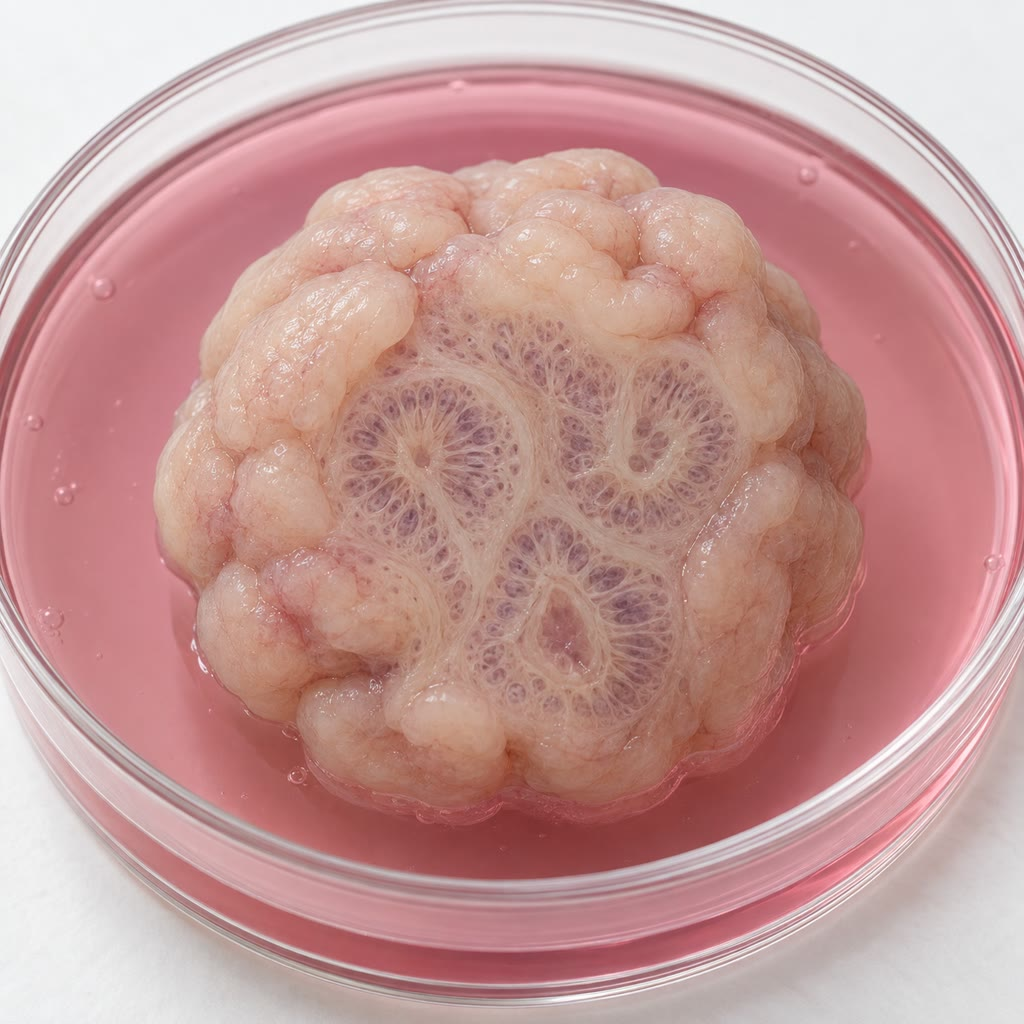
\includegraphics[width=0.4\linewidth]{images/book5/ai/b5-24-brain-organoid.jpg}\hspace{0.04\linewidth}
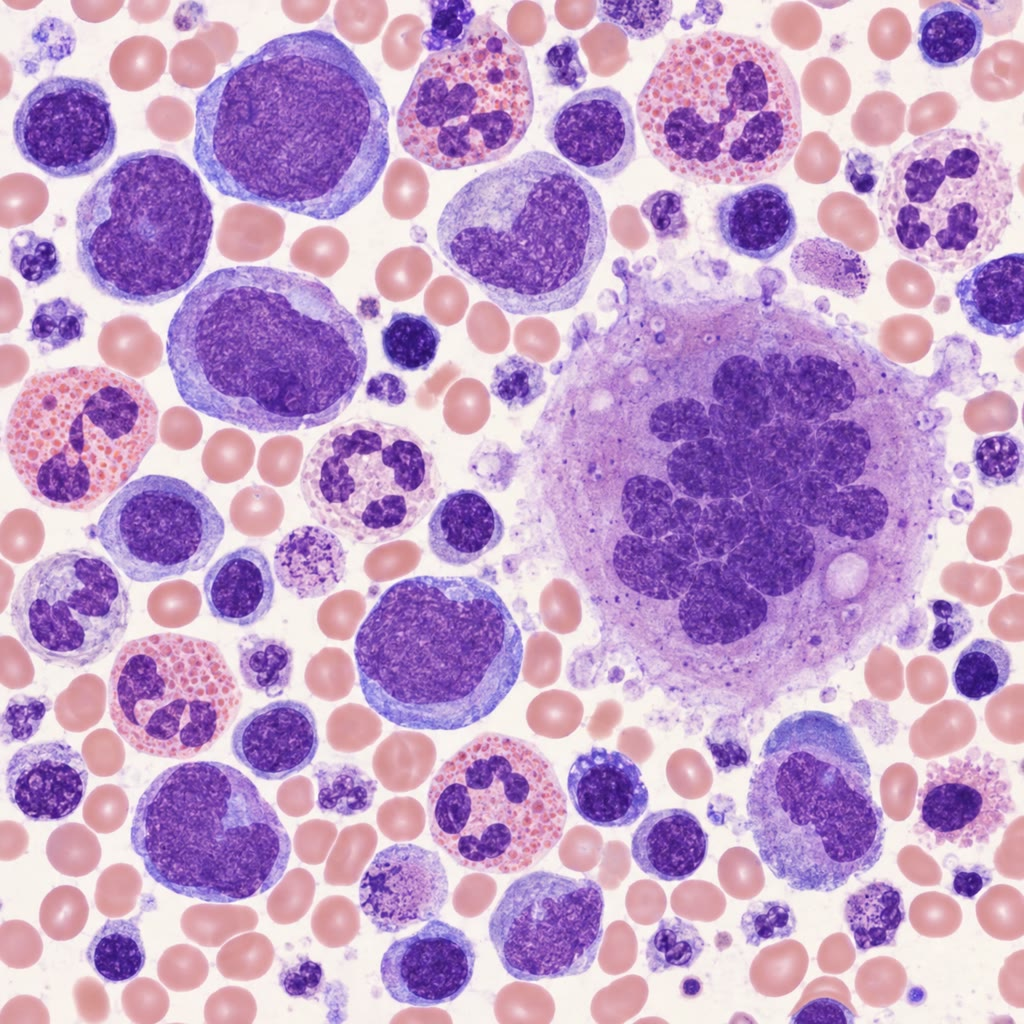
\includegraphics[width=0.4\linewidth]{images/book5/ai/b5-24-bone-marrow-smear.jpg}

{\small Izquierda: un \omterm{def:b3:stem-cells:pluripotency}{organoide} cerebral crecido a partir de células
pluripotentes humanas ---unos pocos milímetros de tejido semejante a
corteza autoorganizado, con cavidades parecidas a ventrículos y
neuronas en capas. Derecha: un frotis de médula ósea, la jerarquía de
la primera figura vista de una vez: blastos, granulocitos en
maduración, precursores de glóbulos rojos y un megacariocito.}
\end{omfigure}

\begin{method}[El rastreo de linajes]\label{met:b3:stem-cells:tracing}
\index{rastreo de linajes}\index{recombinasa Cre}
Para averiguar qué células son las \omterm{def:b3:stem-cells:stem}{células madre} de un tejido: (1)
elíjase un gen que expresen las células candidatas y pónganse bajo su
promotor una recombinasa inducible (Cre-ER, activa solo cuando se da
tamoxifeno); (2) en el mismo animal, un gen indicador que quede
permanentemente activo cuando la recombinasa recorte de él un casete de
parada ---un color que heredan todos sus descendientes; (3) dese una
sola dosis de tamoxifeno para marcar las células candidatas en un
instante; (4) recójase tejido a intervalos y evalúense los clones
marcados: un clon que crece, persiste durante meses y contiene todos
los tipos celulares del tejido procede de una \omterm{def:b3:stem-cells:stem}{célula madre}; un clon que
se desprende en una semana procede de una célula de tránsito. (5) Con
un indicador multicolor, síganse las competencias entre clones. (6)
Pruébese la función directamente matando las células marcadas con un
receptor de toxina expresado bajo el mismo promotor, y véase si el
tejido deja de renovarse.
\end{method}

\section{La regeneración}

\begin{definition}[Cómo regeneran los animales]\label{def:b3:stem-cells:regeneration}
\index{regeneración}\index{neoblasto}\index{blastema}\index{desdiferenciación}\index{crecimiento compensador}
La regeneración sigue tres rutas. \emph{Hydra} y la planaria se apoyan
en \omterm{def:b3:stem-cells:stem}{células madre} pluripotentes adultas: los \emph{neoblastos} de una
planaria, la quinta parte de sus células, son las únicas células que
tiene en división, migran a una herida y reconstruyen cualquier parte
que falte guiados por señales posicionales (un gradiente de Wnt dice al
trozo qué extremo es la cola; bloquéese y un trozo de cola desarrollará
una segunda cabeza). Las salamandras reconstruyen una extremidad a
partir de un \emph{blastema}, un casquete de células en división en el
muñón formado en gran parte por \emph{desdiferenciación}: las fibras
musculares se fragmentan en células mononucleadas, las células del
cartílago y del tejido conjuntivo vuelven a un estado de \omterm{def:b3:stem-cells:stem}{progenitor},
cada una recordando su tejido de origen y su posición a lo largo de la
extremidad, y el blastema vuelve a ejecutar el programa embrionario de
la extremidad bajo la epidermis de la herida y los nervios, cuya
presencia es imprescindible (desnérvese el muñón y no crecerá nada).
Los peces cebra regeneran del mismo modo las aletas y el corazón, y las
células musculares cardíacas supervivientes se dividen para reponer la
quinta parte del ventrículo en un mes. Los mamíferos hacen poco de
esto: el hígado recupera su masa después de que se le retiren dos
tercios, pero por división en su sitio de las células que quedan
(\emph{crecimiento compensador}) y no reconstruyendo los lóbulos
perdidos; la yema de un dedo se regenera en los niños; las astas del
ciervo crecen de nuevo cada año a partir de un periostio de \omterm{def:b3:stem-cells:stem}{células
madre}. Por qué no más es una cuestión de compromisos: la respuesta
mamífera a la herida ---coagulación rápida, \omterm{def:b3:innate-immunity:inflammation}{inflamación}, cicatriz de
fibroblastos--- cierra una herida deprisa frente a la infección y la
pérdida de sangre, y la cicatriz cierra el paso al blastema; y las
células que pueden desdiferenciarse y dividirse a voluntad son células
que pueden volverse \omterm{def:b3:cancer-biology:hallmarks}{cánceres}, un riesgo que un animal longevo y de
sangre caliente quizá no pueda permitirse.
\end{definition}

\begin{omfigure}
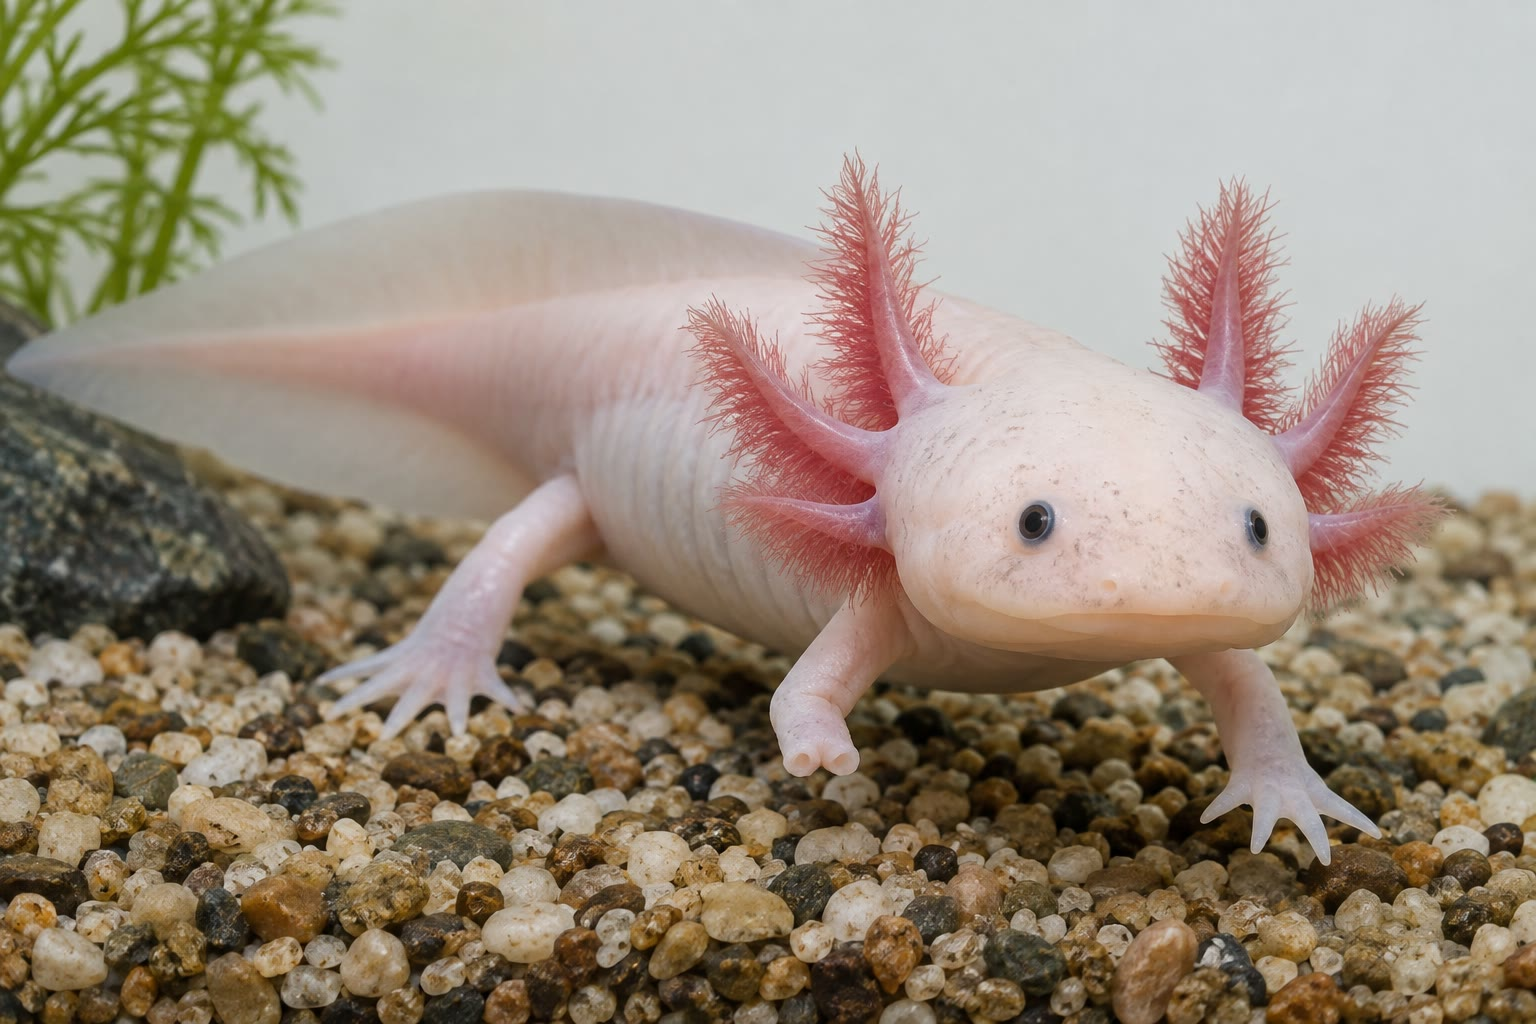
\includegraphics[width=0.46\linewidth]{images/book5/ai/b5-24-axolotl.jpg}\hspace{0.04\linewidth}
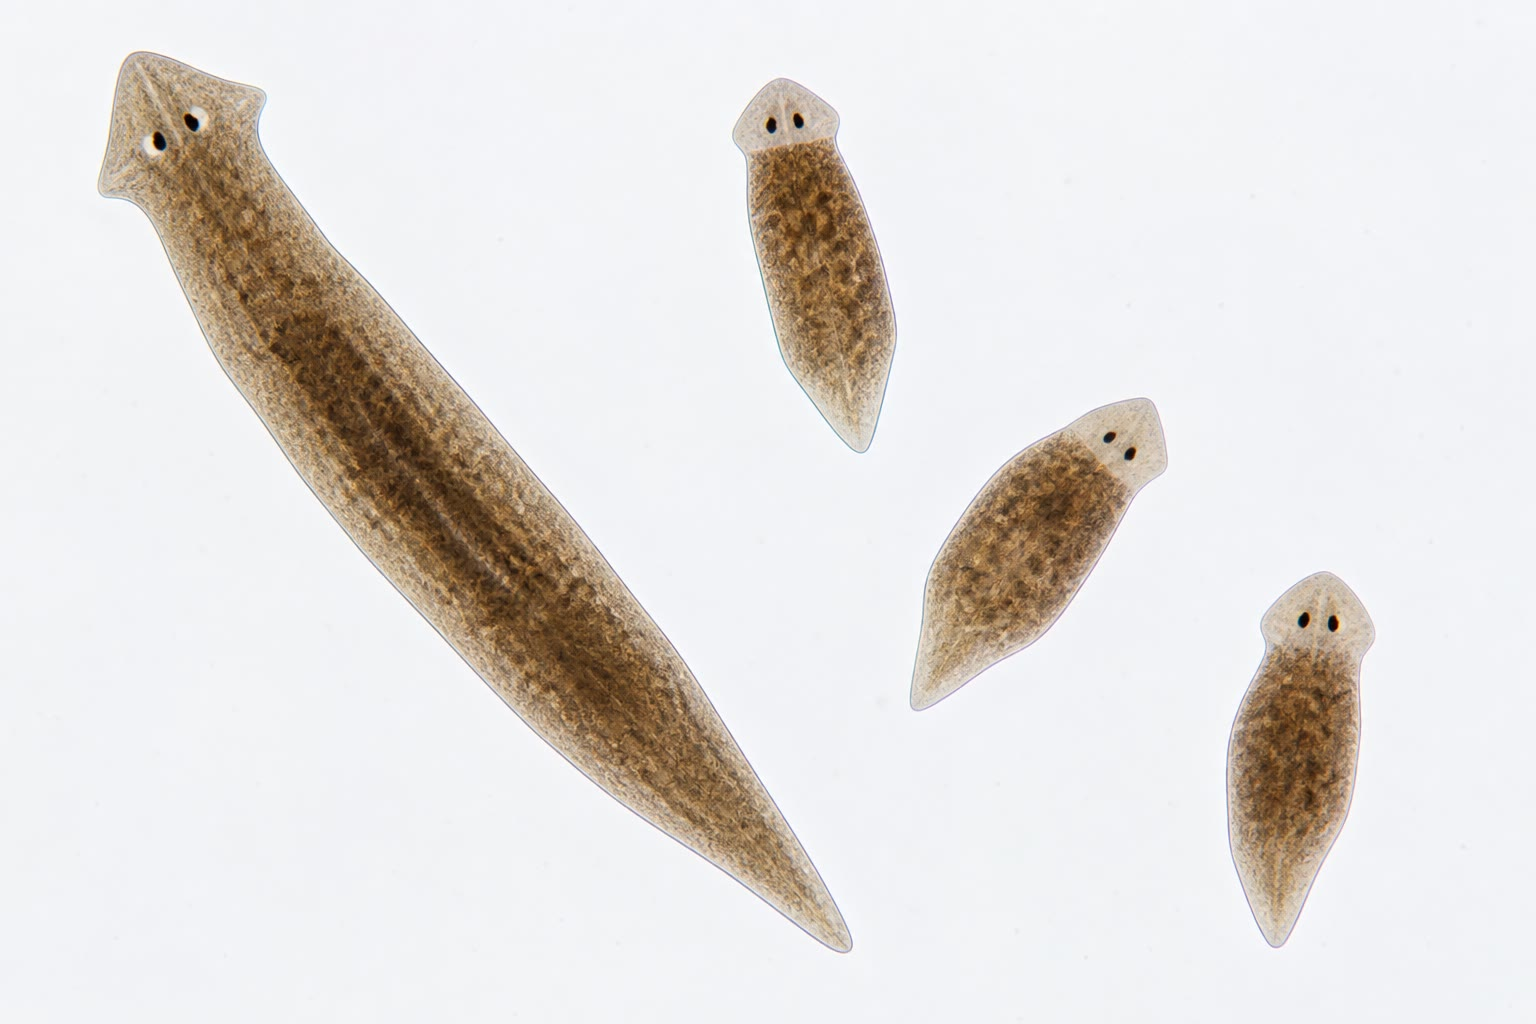
\includegraphics[width=0.46\linewidth]{images/book5/ai/b5-24-planarian-regeneration.jpg}

{\small Izquierda: un ajolote, que regenera una extremidad en dos meses
a partir de un \omterm{def:b3:stem-cells:regeneration}{blastema} de células desdiferenciadas y puede hacerlo
toda su vida. Derecha: una planaria cortada en trozos, cada uno de los
cuales regenera un gusano completo a partir de sus \omterm{def:b3:stem-cells:regeneration}{neoblastos} en dos
semanas.}
\end{omfigure}

\begin{proof}[Evidencia]
Morgan (1898) cortó planarias en 279 trozos y halló que cada uno
regeneraba un gusano entero hasta un límite de aproximadamente una
centésima parte del cuerpo; Reddien y sus colaboradores (2011)
trasplantaron un solo \omterm{def:b3:stem-cells:regeneration}{neoblasto} a un gusano irradiado a dosis letal y
lo restauraron por completo ---una célula, todos los tejidos. Kragl y
sus colaboradores (2009) hicieron ajolotes con los tejidos marcados en
verde de uno en uno y los injertaron en huéspedes sin marcar: tras la
amputación, el músculo verde dio lugar solo a músculo y el cartílago
verde solo a cartílago ---el \omterm{def:b3:stem-cells:regeneration}{blastema} no es una reserva de células
pluripotentes, sino un conjunto de \omterm{def:b3:stem-cells:stem}{progenitores} restringidos a su
linaje, cada uno desdiferenciado solo hasta el \omterm{def:b3:stem-cells:stem}{progenitor} de su propio
tejido. Singer (1952) mostró que una extremidad de salamandra solo se
regenera si llega al muñón un número umbral de fibras nerviosas, y que
desviar un nervio hacia una herida del flanco hacía crecer allí una
extremidad.
\end{proof}

\section{La aritmética del envejecimiento}

\begin{theorem}[Los telómeros y el límite de Hayflick]\label{thm:b3:stem-cells:hayflick}
\index{telómero}\index{límite de Hayflick}\index{problema de la replicación de los extremos}\index{telomerasa}\index{senescencia replicativa}
Cada cromosoma termina en un \emph{telómero}, varias kilobases de la
repetición TTAGGG. Como la ADN-polimerasa no puede completar el último
tramo de la hebra retardada (el \emph{problema de la replicación de los
extremos}), cada división acorta cada telómero en
$\Delta \approx$ \qtyrange{50}{100}{bp}. Partiendo de
$L_{0} \approx \qty{10}{kb}$ y desencadenando la \emph{\omterm{thm:b3:stem-cells:hayflick}{senescencia
replicativa}} ---una parada permanente impuesta por p53--- cuando el
telómero más corto alcanza $L_{\text{crit}} \approx \qty{4}{kb}$, un
linaje celular puede dividirse a lo sumo
\[
n_{\max} = \frac{L_{0} - L_{\text{crit}}}{\Delta} \approx \frac{6000}{50\text{--}100} \approx 60\text{--}120
\]
veces: el \emph{\omterm{thm:b3:stem-cells:hayflick}{límite de Hayflick}}, las cincuenta y tantas
duplicaciones de población que los fibroblastos humanos completan en
cultivo antes de detenerse. La enzima \emph{\omterm{def:b3:cancer-biology:telomerase}{telomerasa}}, una
transcriptasa inversa con molde de ARN, vuelve a alargar los extremos;
está activa en la línea germinal, en las \omterm{def:b3:stem-cells:pluripotency}{células madre embrionarias} y
en muchas adultas, y en el \qty{90}{\%} de los \omterm{def:b3:cancer-biology:hallmarks}{cánceres}, que han
escapado del límite volviéndola a encender. Una \omterm{def:b3:stem-cells:stem}{célula madre} que se
divide $d$ veces al año con la \omterm{def:b3:cancer-biology:telomerase}{telomerasa} compensando una fracción $f$
de la pérdida tiene $n_{\max} = (L_{0} - L_{\text{crit}})/[(1 - f)\Delta]$
divisiones, y una vida de $n_{\max}/d$ años: con $f = 0.7$, $\Delta
= 60$ y $d = 1$, unos 330 años para una \omterm{def:b3:stem-cells:stem}{célula madre} hematopoyética
---pero sus \omterm{def:b3:stem-cells:stem}{progenitores}, con la \omterm{def:b3:cancer-biology:telomerase}{telomerasa} apagada y veinte divisiones
hasta un glóbulo rojo, gastan la quinta parte de su reserva en cada
linaje, y por eso los glóbulos de las personas mayores tienen telómeros
más cortos que los de las jóvenes, en unos \qty{30}{bp} al año.
\end{theorem}
\begin{proof}
La pérdida por división es una longitud fija, de modo que la longitud
del telómero cae linealmente con el número de divisiones,
$L_{n} = L_{0} - n\Delta$, y alcanza $L_{\text{crit}}$ en
$n = (L_{0} - L_{\text{crit}})/\Delta$; con compensación parcial, la
pérdida neta por división es $(1 - f)\Delta$. Hayflick y Moorhead
(1961) mostraron que los fibroblastos humanos normales se detienen tras
unas cincuenta duplicaciones sean cuales sean las condiciones de
cultivo, que las células congeladas tras veinte duplicaciones y
descongeladas completan solo las treinta restantes ---cuentan
divisiones, no tiempo--- y que el límite es menor para células de
donantes mayores. Harley, Futcher y Greider (1990) midieron el
acortamiento de los telómeros con las duplicaciones en cultivo y con la
edad del donante; Bodnar y sus colaboradores (1998) introdujeron
\omterm{def:b3:cancer-biology:telomerase}{telomerasa} en células normales y estas se dividieron más allá del
límite indefinidamente sin volverse cancerosas, lo que estableció el
telómero como el reloj.
\end{proof}

\begin{omfigure}
\begin{tikzpicture}
\begin{axis}[
  width=0.62\linewidth, height=5.4cm,
  axis x line=bottom, axis y line=left,
  xmin=0, xmax=120, ymin=0, ymax=11,
  xlabel={duplicaciones de población}, ylabel={longitud del telómero (kb)},
  xlabel style={font=\small, at={(axis description cs:0.5,-0.12)}, anchor=north}, ylabel style={font=\small},
  tick label style={font=\small}, xtick={0,30,60,90,120}, ytick={4,7,10},
  clip=false,
]
\addplot[very thick, omDef, domain=0:60, samples=2] {10-0.1*x};
\addplot[very thick, omThm, domain=0:120, samples=2] {10-0.05*x};
\addplot[very thick, omMeth!70!black, domain=0:120, samples=2] {10-0.015*x};
\draw[dashed, gray] (axis cs:0,4) -- (axis cs:120,4); \node[font=\scriptsize, gray, anchor=north west] at (axis cs:2,3.9) {senescencia en $L_{\text{crit}} = \qty{4}{kb}$};
\node[font=\scriptsize, omDef, anchor=south west] at (axis cs:63,4.3) {$\Delta = \qty{100}{bp}$: 60 duplicaciones};
\node[font=\scriptsize, omThm, anchor=west] at (axis cs:70,8.0) {$\Delta = \qty{50}{bp}$: 120};
\node[font=\scriptsize, omMeth!70!black, anchor=south west, align=left] at (axis cs:78,9.3) {telomerasa que compensa\\el \qty{70}{\%}: 400};
\fill[omDef] (axis cs:60,4) circle (2pt); \fill[omThm] (axis cs:120,4) circle (2pt);
\end{axis}
\end{tikzpicture}

{\small Los telómeros como contador de divisiones. Una pérdida fija por
división da una recta; donde esta cruza la longitud crítica, el linaje
se detiene. La \omterm{def:b3:cancer-biology:telomerase}{telomerasa} aplana la pendiente y, plenamente activa,
abole el límite ---en la línea germinal y en los \omterm{def:b3:cancer-biology:hallmarks}{cánceres}.}
\end{omfigure}

\begin{proposition}[La ley de Gompertz]\label{prop:b3:stem-cells:gompertz}
\index{ley de Gompertz}\index{tasa de mortalidad}\index{marcas del envejecimiento}\index{célula senescente}
Por encima de los treinta años, la tasa humana de mortalidad $\mu(t)$
---la probabilidad de morir en el año siguiente--- se duplica cada ocho
años: $\mu(t) =
\mu_{0}\,\mathrm{e}^{\gamma(t - t_{0})}$ con $\gamma = \ln 2/8 \approx
\qty{0.087}{yr^{-1}}$ (Gompertz, 1825). La supervivencia hasta la edad
$t$ es entonces
\[
S(t) = \exp\!\Bigl[-\frac{\mu_{0}}{\gamma}\bigl(\mathrm{e}^{\gamma(t - t_{0})} - 1\bigr)\Bigr],
\]
una curva plana durante décadas y que cae después en picado, con una
vida mediana $t_{1/2} = t_{0} + \gamma^{-1}\ln(1 + \gamma\ln 2/\mu_{0})$:
para $\mu_{0} = 10^{-3}$ al año a los treinta, unos $30 + 47 = 77$
años. La misma ley, con otras constantes, vale para los ratones (con un
tiempo de duplicación de tres meses), los perros, las moscas y los
gusanos: el envejecimiento es una subida exponencial de la
vulnerabilidad, no un reloj que se para. La biología que hay tras el
exponente es un conjunto de \emph{marcas} que interaccionan: daño
acumulado en el ADN y deriva \omterm{def:b3:chromatin-epigenetics:epigenetics}{epigenética}, desgaste de los telómeros,
pérdida de la proteostasis, declive mitocondrial, agotamiento de las
reservas de \omterm{def:b3:stem-cells:stem}{células madre}, acumulación de \emph{\omterm{prop:b3:stem-cells:gompertz}{células senescentes}}
que ya no se dividen pero segregan señales inflamatorias, e
\omterm{def:b3:innate-immunity:inflammation}{inflamación} crónica; en ratones, eliminar las \omterm{prop:b3:stem-cells:gompertz}{células senescentes} o
restringir las calorías alarga la vida, y en gusanos una sola mutación
de la vía parecida a la de la \omterm{def:b3:endocrinology:glucose}{insulina} la duplica. Si el exponente
puede bajarse en los seres humanos, en lugar de la constante $\mu_{0}$,
que la medicina ha reducido diez veces en un siglo, es la cuestión
abierta.
\end{proposition}
\begin{proof}
Si $\mu$ es el riesgo instantáneo,
$\mathrm{d}S/\mathrm{d}t = -\mu(t)S$, de modo que $\ln S =
-\int_{t_{0}}^{t}\mu = -(\mu_{0}/\gamma)(\mathrm{e}^{\gamma(t-t_{0})} -
1)$. Haciendo $S = 1/2$: $\mathrm{e}^{\gamma(t-t_{0})} = 1 + \gamma\ln 2/
\mu_{0}$, de donde la mediana; con $\gamma = 0.087$ y $\mu_{0} =
10^{-3}$, $\ln(1 + 60) = 4.1$ y $t - t_{0} = 47$. La ley empírica es el
ajuste de Gompertz a las tablas de mortalidad inglesas; que describa a
tantas especies con una forma común y constantes propias de cada una se
admite aquí como resumen de un siglo de demografía.
\end{proof}

\begin{omfigure}
\begin{tikzpicture}
\begin{semilogyaxis}[
  width=0.5\linewidth, height=5.2cm,
  axis x line=bottom, axis y line=left,
  xmin=20, xmax=100, ymin=0.0003, ymax=1,
  xlabel={edad (años)}, ylabel={tasa de mortalidad anual},
  xlabel style={font=\small, at={(axis description cs:0.5,-0.12)}, anchor=north}, ylabel style={font=\small},
  tick label style={font=\small}, xtick={30,50,70,90}, ytick={0.001,0.01,0.1,1}, yticklabels={0.001,0.01,0.1,1},
  clip=false,
]
\addplot[very thick, omDef, domain=30:100, samples=2] {0.001*exp(0.0866*(x-30))};
\node[font=\scriptsize, omDef, anchor=north west, align=left] at (axis cs:32,0.3) {$\mu = \mu_{0}\,\mathrm{e}^{\gamma(t-30)}$\\se duplica cada 8 años};
\end{semilogyaxis}
\begin{axis}[
  at={(0.55\linewidth,0)}, anchor=south west,
  width=0.43\linewidth, height=5.2cm,
  axis x line=bottom, axis y line=left,
  xmin=20, xmax=110, ymin=0, ymax=1.05,
  xlabel={edad (años)}, ylabel={fracción superviviente},
  xlabel style={font=\small, at={(axis description cs:0.5,-0.12)}, anchor=north}, ylabel style={font=\small},
  tick label style={font=\small}, xtick={30,50,77,100}, ytick={0.5,1},
  clip=false,
]
\addplot[very thick, omThm, domain=30:110, samples=80] {exp(-(0.001/0.0866)*(exp(0.0866*(x-30))-1))};
\draw[dashed, gray] (axis cs:77,0) -- (axis cs:77,0.5) -- (axis cs:20,0.5);
\node[font=\scriptsize, omThm, anchor=north east, align=right] at (axis cs:75,0.45) {mediana\\77 años};
\end{axis}
\end{tikzpicture}

{\small La \omterm{prop:b3:stem-cells:gompertz}{ley de Gompertz}. Izquierda: en un eje logarítmico la \omterm{prop:b3:stem-cells:gompertz}{tasa de
mortalidad} es una recta a partir de los treinta. Derecha: la curva de
supervivencia que se sigue ---una meseta y luego un acantilado, con la
mediana allí donde la integral del riesgo alcanza $\ln 2$.}
\end{omfigure}

\begin{remark}[La renovación y su precio]\label{rem:b3:stem-cells:remark}
Un cuerpo que se renueva ha de conservar células capaces de dividirse
indefinidamente, y las células capaces de dividirse indefinidamente son
la materia del \omterm{def:b3:cancer-biology:hallmarks}{cáncer}; un cuerpo que se protege del \omterm{def:b3:cancer-biology:hallmarks}{cáncer} contando
divisiones e imponiendo la \omterm{def:b3:cell-cycle-apoptosis:other}{senescencia} ha de quedarse, con el tiempo,
sin células capaces de dividirse. La jerarquía de \omterm{def:b3:stem-cells:stem}{células madre} es una
solución ---pocas células lentas protegidas en \omterm{def:b3:stem-cells:stem}{nichos}, muchas células
rápidas que pronto mueren--- y el \omterm{thm:b3:stem-cells:hayflick}{límite de Hayflick} es otra, y la
exponencial de Gompertz es la suma de sus costes. La salamandra paga de
otro modo: tolera células que se desdiferencian y regenera una pata, y
es de sangre fría, lenta y rara vez vive lo bastante para pagar la
factura del \omterm{def:b3:cancer-biology:hallmarks}{cáncer}. Las células con las que uno nació no son, en su
mayor parte, las que tiene; las que hicieron los repuestos son las que
hay que conservar.
\end{remark}

\section{Ejercicios}

\begin{exercise}[$\star$]\label{exo:b3:stem-cells:1}
Defínanse la \omterm{def:b3:stem-cells:stem}{autorrenovación}, la potencia, el \omterm{def:b3:stem-cells:stem}{nicho} y la \omterm{def:b3:stem-cells:stem}{célula
amplificadora de tránsito}, y dese un ejemplo de cada uno en el
intestino.
\end{exercise}

\begin{exercise}[$\star$]\label{exo:b3:stem-cells:2}
¿Qué mostró el ensayo de colonias esplénicas, y qué propiedad de una
\omterm{def:b3:stem-cells:stem}{célula madre} exigió un segundo ratón para demostrarse?
\end{exercise}

\begin{exercise}[$\star$]\label{exo:b3:stem-cells:3}
Nómbrense los cuatro factores de Yamanaka y explíquese por qué la
\omterm{def:b3:stem-cells:pluripotency}{reprogramación} tarda semanas y funciona en una milésima de las células.
\end{exercise}

\begin{exercise}[$\star$]\label{exo:b3:stem-cells:4}
Contrástense las rutas de la planaria y de la salamandra hacia la
\omterm{def:b3:stem-cells:regeneration}{regeneración}, y dígase qué mostraron los injertos de Kragl sobre el
\omterm{def:b3:stem-cells:regeneration}{blastema}.
\end{exercise}

\begin{exercise}[$\star\star$]\label{exo:b3:stem-cells:5}
Los telómeros parten de \qty{11}{kb}, la \omterm{def:b3:cell-cycle-apoptosis:other}{senescencia} llega a
\qty{5}{kb} y la pérdida es de \qty{75}{bp} por división. ¿\omterm{thm:b3:stem-cells:hayflick}{Límite de
Hayflick}? Las células de un donante de 70 años tienen \qty{8}{kb}:
¿duplicaciones restantes? Si la \omterm{def:b3:cancer-biology:telomerase}{telomerasa} compensa el \qty{60}{\%} de
la pérdida, ¿límite?
\end{exercise}

\begin{exercise}[$\star\star$]\label{exo:b3:stem-cells:6}
Una cripta tiene 14 \omterm{def:b3:stem-cells:stem}{células madre} que se dividen una vez al día y
alimentan células de tránsito que se dividen 4 veces más, y la cripta
suministra \num{300} células al día a su vellosidad. Compruébese la
aritmética: ¿cuántas divisiones de \omterm{def:b3:stem-cells:stem}{células madre} al día producen hijas
que se diferencian, y a cuántas \omterm{def:b3:stem-cells:stem}{células madre} equivale eso en
divisiones?
\end{exercise}

\begin{exercise}[$\star\star$]\label{exo:b3:stem-cells:7}
El cuerpo fabrica $2\times 10^{11}$ glóbulos rojos al día, cada uno
producto de unas 20 divisiones desde una \omterm{def:b3:stem-cells:stem}{célula madre}. ¿Cuántas
divisiones de \omterm{def:b3:stem-cells:stem}{células madre} al día exige eso y, con \num{10000} \omterm{def:b3:stem-cells:stem}{células
madre}, cada cuánto se divide cada una? Compárese con el ``alrededor de
una vez al año'' observado y explíquese la discrepancia.
\end{exercise}

\begin{exercise}[$\star\star$]\label{exo:b3:stem-cells:8}
Con $\gamma = \qty{0.087}{yr^{-1}}$ y $\mu_{0} = 10^{-3}$ a los treinta,
calcúlense la \omterm{prop:b3:stem-cells:gompertz}{tasa de mortalidad} a los 50, 70 y 90 años, la
supervivencia hasta los 70 y los 90, y la vida mediana. ¿Qué le hace a
la mediana reducir $\mu_{0}$ a la mitad? ¿Y reducir $\gamma$ a la mitad?
\end{exercise}

\begin{exercise}[$\star\star$]\label{exo:b3:stem-cells:9}
Se extirpan dos tercios del hígado de una rata. Los hepatocitos
restantes, que se dividen todos, restauran la masa en diez días.
¿Cuántas divisiones necesita cada uno? ¿Por qué se llama a esto
\omterm{def:b3:stem-cells:regeneration}{crecimiento compensador} y no \omterm{def:b3:stem-cells:regeneration}{regeneración}, y qué \emph{no} reconstruye
el hígado?
\end{exercise}

\begin{exercise}[$\star\star\star$]\label{exo:b3:stem-cells:10}
\omterm{prop:b3:stem-cells:crypt}{Deriva neutra}: $N$ \omterm{def:b3:stem-cells:stem}{células madre} de un \omterm{def:b3:stem-cells:stem}{nicho} se dividen de forma
simétrica; en cada suceso una célula se divide y otra se pierde al
azar, de modo que el número de un clon dado hace un paseo aleatorio
entre $0$ y $N$. Arguméntese que la probabilidad de que un clon de $k$
células acabe apoderándose del \omterm{def:b3:stem-cells:stem}{nicho} es $k/N$, y que con $N = 14$ un
clon de una sola célula tiene una probabilidad de $1/14$. ¿Qué predice
esto para el destino de una \omterm{def:b3:stem-cells:stem}{célula madre} portadora de una mutación
neutra nueva?
\end{exercise}

\begin{exercise}[$\star\star\star$]\label{exo:b3:stem-cells:11}
Una mutación da a un clon de \omterm{def:b3:stem-cells:stem}{células madre} una ventaja del \qty{10}{\%}
en la competencia de \cref{exo:b3:stem-cells:10}. Explíquese
cualitativamente por qué su probabilidad de imponerse sube muy por
encima de $k/N$, por qué las criptas y la médula de las personas
mayores están cada vez más dominadas por unos pocos clones
(hematopoyesis clonal), y por qué esto es un primer paso hacia el
\omterm{def:b3:cancer-biology:hallmarks}{cáncer} sin ser \omterm{def:b3:cancer-biology:hallmarks}{cáncer}.
\end{exercise}

\begin{exercise}[$\star\star\star$]\label{exo:b3:stem-cells:12}
Supóngase que el exponente $\gamma$ de Gompertz refleja un ritmo de
acumulación de daño y la constante $\mu_{0}$ el ambiente. La medicina
ha reducido $\mu_{0}$ diez veces desde 1900 sin cambiar $\gamma$.
Calcúlese la ganancia de vida mediana que da esa reducción de diez
veces, y la ganancia adicional de otra reducción de diez veces;
explíquese por qué los rendimientos son decrecientes, y qué haría en su
lugar una reducción del \qty{20}{\%} de $\gamma$.
\end{exercise}

\section{Problema: las células con las que naciste}

\begin{problem}[{Problema de fin de semana --- la renovación de un
cuerpo en números: la jerarquía de la sangre y lo que pide a sus
células madre, la deriva de la cripta, el reloj del telómero y cómo lo
gastan la telomerasa y los progenitores, la curva de Gompertz de la
población, y los compromisos que acepta un animal que regenera, para
terminar en el recuento de Hayflick, la reserva vitalicia de una célula
madre y la vida mediana}]
\label{pb:b3:stem-cells:1}
Datos: glóbulos rojos $2.5\times 10^{11}$ al día y granulocitos
$10^{11}$ al día; $20$ divisiones desde la \omterm{def:b3:stem-cells:stem}{célula madre} hasta la célula
madura; \num{10000} \omterm{def:b3:stem-cells:stem}{células madre} hematopoyéticas. Telómeros:
$L_{0} = \qty{10}{kb}$, $L_{\text{crit}} = \qty{4}{kb}$,
$\Delta = \qty{60}{bp}$ por división; la \omterm{def:b3:cancer-biology:telomerase}{telomerasa} de las \omterm{def:b3:stem-cells:stem}{células
madre} compensa $f = 0.7$, y no hay ninguna en los \omterm{def:b3:stem-cells:stem}{progenitores}. Cripta:
$N = 14$ \omterm{def:b3:stem-cells:stem}{células madre}, una división al día. Gompertz: $\mu_{0} =
10^{-3}$ al año a los 30, $\gamma = \qty{0.087}{yr^{-1}}$. Extremidad
de ajolote: \qty{40}{mm} regenerados en \qty{60}{d}; \omterm{def:b3:stem-cells:regeneration}{blastema} de
$10^{5}$ células que crece hasta $10^{8}$.

\medskip
\noindent\textbf{Parte I --- La sangre.}
\begin{enumerate}
  \item Células producidas al día en total, y por segundo.
  \item Cada célula madura es el final de $20$ divisiones: ¿cuántas
        células resultan de una sola hija comprometida de una \omterm{def:b3:stem-cells:stem}{célula
        madre}? ¿Cuántas hijas comprometidas hacen falta al día?
  \item Con \num{10000} \omterm{def:b3:stem-cells:stem}{células madre}, ¿cuántas divisiones que producen
        diferenciación por \omterm{def:b3:stem-cells:stem}{célula madre} y día implica eso? ¿Y al año?
  \item La división medida de las \omterm{def:b3:stem-cells:stem}{células madre} es de alrededor de una
        vez al año. Concíliese: ¿qué han de hacer los \omterm{def:b3:stem-cells:stem}{progenitores} que
        el cálculo de la pregunta~3 daba por hecho que hacían las
        \omterm{def:b3:stem-cells:stem}{células madre}?
  \item Los \omterm{def:b3:stem-cells:stem}{progenitores} no tienen \omterm{def:b3:cancer-biology:telomerase}{telomerasa}. Partiendo de
        \qty{10}{kb}, ¿qué longitud de telómero alcanza un precursor de
        glóbulo rojo tras sus $20$ divisiones? ¿Importa que esté por
        encima de $L_{\text{crit}}$?
  \item Una \omterm{def:b3:stem-cells:stem}{célula madre} que se divide una vez al año con $f = 0.7$:
        pérdida neta por división, divisiones hasta la \omterm{def:b3:cell-cycle-apoptosis:other}{senescencia} y
        años. Coméntese.
\end{enumerate}

\medskip
\noindent\textbf{Parte II --- La cripta.}
\begin{enumerate}[resume]
  \item Divisiones por cripta y día en el piso de las \omterm{def:b3:stem-cells:stem}{células madre}; si
        la mitad de los sucesos reemplaza a una \omterm{def:b3:stem-cells:stem}{célula madre} perdida y
        la otra mitad alimenta la zona de tránsito, ¿cuántas células
        comprometidas al día, y cuántas células de vellosidad tras $4$
        divisiones de tránsito?
  \item La probabilidad de que un clon de una sola célula se imponga es
        $1/N$. El tiempo esperado hasta la monoclonalidad es del orden
        de $N^{2}$ sucesos de división por célula; estímese en días y
        compárese con las observaciones del confeti (meses).
  \item Una \omterm{def:b3:stem-cells:stem}{célula madre} adquiere una mutación. ¿Probabilidad de que
        acabe fijada en su cripta? ¿En cuántas de los $10^{7}$ criptas
        de un colon quedaría fijada una mutación surgida una vez por
        cripta?
  \item ¿Por qué protege más del \omterm{def:b3:cancer-biology:hallmarks}{cáncer} la deriva de una cripta que un
        tejido en el que todas las \omterm{def:b3:stem-cells:stem}{células madre} se dividan de forma
        asimétrica de por vida?
  \item Cuando la irradiación mata las \omterm{def:b3:stem-cells:stem}{células madre}, las células de
        tránsito revierten y vuelven a llenar el \omterm{def:b3:stem-cells:stem}{nicho}. ¿Qué dice esto
        sobre dónde reside el carácter de madre?
  \item Bosquéjese el experimento de \omterm{met:b3:stem-cells:tracing}{rastreo de linajes} que distingue
        la deriva simétrica de la \omterm{def:b3:stem-cells:stem}{división asimétrica}, y los dos
        resultados.
\end{enumerate}

\medskip
\noindent\textbf{Parte III --- El reloj.}
\begin{enumerate}[resume]
  \item \omterm{thm:b3:stem-cells:hayflick}{Límite de Hayflick} para un linaje somático sin \omterm{def:b3:cancer-biology:telomerase}{telomerasa}.
  \item Un cultivo de fibroblastos se congela tras $25$ duplicaciones y
        se descongela una década después: ¿duplicaciones restantes? ¿Qué
        muestra esto sobre lo que cuenta la célula?
  \item Los telómeros de los leucocitos se acortan \qty{30}{bp} al año
        en los adultos. Partiendo de \qty{8}{kb} a los veinte, ¿cuándo
        alcanzarían $L_{\text{crit}}$? Compárese con la vida y
        coméntese.
  \item Añadir \omterm{def:b3:cancer-biology:telomerase}{telomerasa} a fibroblastos normales les permite superar el
        límite sin volverse cancerosos. La \omterm{def:b3:cancer-biology:telomerase}{telomerasa} está activa en el
        \qty{90}{\%} de los \omterm{def:b3:cancer-biology:hallmarks}{cánceres}. Concíliense ambas afirmaciones.
  \item Calcúlense la \omterm{prop:b3:stem-cells:gompertz}{tasa de mortalidad} de Gompertz a los 40, 60, 80 y
        100 años, y la supervivencia hasta cada edad.
  \item Vida mediana; y la edad a la que sobrevive el \qty{10}{\%}.
\end{enumerate}

\medskip
\noindent\textbf{Parte IV --- Regenerar.}
\begin{enumerate}[resume]
  \item Ajolote: velocidad media de \omterm{def:b3:stem-cells:regeneration}{regeneración} en mm/día;
        duplicaciones para que el \omterm{def:b3:stem-cells:regeneration}{blastema} pase de $10^{5}$ a $10^{8}$
        células, y tiempo medio de duplicación a lo largo de 60 días.
  \item Si las células desdiferenciadas se dividieran como las del
        \omterm{def:b3:stem-cells:regeneration}{blastema} durante toda la vida y una división acarreara una
        probabilidad de $10^{-9}$ por célula de una mutación oncogénica,
        ¿cuántas mutaciones así surgen en una \omterm{def:b3:stem-cells:regeneration}{regeneración}? ¿Por qué el
        ajolote casi nunca tiene \omterm{def:b3:cancer-biology:hallmarks}{cáncer}, y por qué un mamífero podría no
        salir indemne?
  \item Desnervar el muñón detiene la \omterm{def:b3:stem-cells:regeneration}{regeneración}. Propóngase un
        experimento que muestre que el nervio aporta un factor
        difusible, y una posible identidad del factor.
  \item Un trozo de cola de planaria desarrolla una segunda cola en
        lugar de una cabeza cuando se silencia un inhibidor de Wnt.
        Explíquese con un gradiente y la memoria posicional del trozo.
  \item Hígado humano tras una resección de dos tercios: fracción de
        hepatocitos que han de dividirse una vez, y dos, para restaurar
        la masa. ¿Por qué el resultado es un hígado que funciona pero
        con la forma equivocada?
  \item ¿Por qué tendría una curva de Gompertz distinta un cuerpo que
        regenerase como un ajolote, y en qué sentido?
  \item Resúmase: el recuento de Hayflick (pregunta~13), las divisiones
        y los años de una \omterm{def:b3:stem-cells:stem}{célula madre} asistida por \omterm{def:b3:cancer-biology:telomerase}{telomerasa}
        (pregunta~6) y la vida mediana (pregunta~18).
\end{enumerate}
\end{problem}
